\documentclass[sigconf, screen, review]{acmart}
\AtBeginDocument{\providecommand\BibTeX{{Bib\TeX}}}
\setcopyright{none}\copyrightyear{2026}\acmYear{2026}\acmDOI{}
\acmConference[MICRO 2026]{The 59th IEEE/ACM International Symposium on Microarchitecture}{November 2026}{Austin, TX, USA}
\acmISBN{}\settopmatter{printfolios=true}\settopmatter{printacmref=false}
\author{Anonymous Author(s)}\affiliation{\institution{Under Review}\country{Anonymous}}
\usepackage{multirow}\usepackage{enumitem}\usepackage{tikz}
\usetikzlibrary{shapes.geometric,arrows.meta,positioning,fit,backgrounds,patterns,decorations.pathreplacing}
\usepackage{pgfplots}\pgfplotsset{compat=1.18}\usepgfplotslibrary{groupplots}\usetikzlibrary{plotmarks}
\newcommand{\todo}[1]{}
\begin{document}
\title{A Survey of High-Level Modeling and Simulation Methods for Modern Machine Learning Workloads}
\begin{abstract}
We survey 25 performance modeling tools from 53 papers (2016--2026) and evaluate ten---NeuSight, ASTRA-sim, VIDUR, Timeloop, nn-Meter with full experiments, plus MAESTRO, Paleo, Habitat, Accel-Sim with deployment testing---across 146 GPU configurations, collective benchmarks, LLM serving, energy validation, and reproducibility testing. Three findings emerge: (1)~self-reported accuracy is unreliable---NeuSight claims 2.3\% MAPE but we measure 5.87--27.10\%, while nn-Meter produces no output due to dependency rot; (2)~the five tools are complementary but disjoint, motivating a unified pipeline; (3)~the kernel-to-model composition gap (2--9\% kernel error growing to 10--28\% model error) dominates total error, yet no tool addresses this layer.
\end{abstract}\keywords{ML workload performance prediction, DNN accelerator modeling, GPU simulation, distributed training simulation, LLM inference serving, design space exploration, survey}\maketitle
\section{Introduction}\label{sec:introduction}
Domain-specific architectures~\cite{hennessy2019golden,tpuv1_2017,tpuv4_2023} make performance prediction critical, yet no prior work examines \emph{why} certain approaches succeed or how errors propagate; prior surveys cover ML techniques for modeling~\cite{granite2022}, specific hardware, or distributed training simulators~\cite{svedassurvey2025}. We contribute: (1)~the \textbf{MLPerf-Survey-2026} benchmark suite of \textbf{36 scenarios} where 56\% of scenarios lack tool support; (2)~\textbf{third-party evaluation} showing claimed error rates are overstated by $2$--$4\times$; (3)~a \textbf{unified pipeline} identifying the composition gap; and (4)~a \textbf{research agenda} for composition modeling and continuous validation.
\begin{figure}[t]
\centering\resizebox{\columnwidth}{!}{%
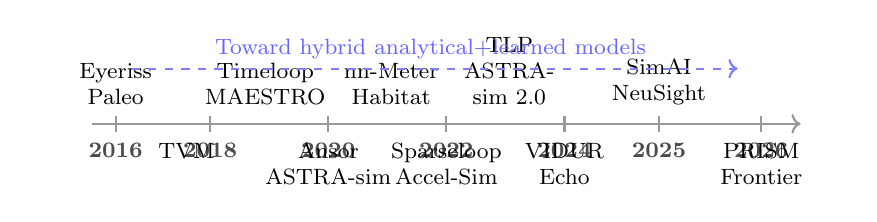
\begin{tikzpicture}[yearnode/.style={font=\footnotesize\bfseries, text=black!70}, eventnode/.style={font=\footnotesize, text width=2cm, align=center}]
\draw[thick, ->, black!40] (0,0) -- (9,0); \foreach \x/\year in {0.3/2016, 1.5/2018, 3/2020, 4.5/2022, 6/2024, 7.2/2025, 8.5/2026} { \draw[thick, black!40] (\x,-0.1) -- (\x,0.1); \node[yearnode, below] at (\x,-0.12) {\year}; }
\node[eventnode, above] at (0.3,0.12) {Eyeriss\\Paleo}; \node[eventnode, below] at (1.2,-0.12) {TVM}; \node[eventnode, above] at (2.2,0.12) {Timeloop\\MAESTRO}; \node[eventnode, below] at (3,-0.12) {Ansor\\ASTRA-sim}; \node[eventnode, above] at (3.8,0.12) {nn-Meter\\Habitat}; \node[eventnode, below] at (4.5,-0.12) {Sparseloop\\Accel-Sim}; \node[eventnode, above] at (5.3,0.12) {TLP\\ASTRA-sim 2.0}; \node[eventnode, below] at (6,-0.12) {VIDUR\\Echo}; \node[eventnode, above] at (7.2,0.12) {SimAI\\NeuSight}; \node[eventnode, below] at (8.5,-0.12) {PRISM\\Frontier};
\draw[thick, ->, blue!50, dashed] (0.5,0.7) -- (8.2,0.7); \node[font=\footnotesize, text=blue!60, above] at (4.3,0.7) {Toward hybrid analytical+learned models};
\end{tikzpicture}}\caption{Evolution of performance modeling tools (2016--2026).}\label{fig:timeline}\end{figure}
\section{Survey Methodology}\label{sec:methodology}
From 287 candidates on ACM DL, IEEE Xplore, Semantic Scholar, and arXiv, 53 papers (2016--2026) plus 12 foundational works were classified by methodology, platform, and abstraction level~\cite{rakhshanfar2021survey}, excluding proprietary tools, infrastructure~\cite{binkert2011gem5,sst2012}, compilers~\cite{halide2013,mlir2020,triton2019}, and schedulers~\cite{pollux2021,sia2023}.
\textbf{Background.}
ML workloads are computation graphs~\cite{pytorch2019,tensorflow2016} where performance depends on dataflow, KV cache management~\cite{vllm2023}, and compute--memory--network balance; LLM inference splits into compute-bound prefill and memory-bound decode~\cite{splitwise2024,sarathi2024,orca2022}. Five modeling types span accuracy--speed trade-offs: \textbf{analytical}~\cite{williams2009roofline,rooflinellm2024} ($\mu$s), \textbf{cycle-accurate}~\cite{gpgpusim2009,accelsim2020,dissectinggpu2025} ($10^3$--$10^4\times$ slowdown), \textbf{trace-driven}~\cite{astrasim2023,vidur2024} (min.), \textbf{ML-augmented}~\cite{nnmeter2021} (ms), and \textbf{hybrid}~\cite{neusight2025,habitat2021}.
\section{Taxonomy}\label{sec:taxonomy}
We organize the literature by \emph{methodology type}, \emph{target platform}, and \emph{abstraction level} (Table~\ref{tab:taxonomy-matrix}).\begin{table*}[t]
\centering\caption{Methodology taxonomy: coverage matrix and trade-off profile. \textbf{0} = research gap.}\label{tab:taxonomy-matrix}\footnotesize\begin{tabular}{l|ccccc|cccc}\toprule
 & \textbf{DNN} & & \textbf{Distrib.} & \textbf{Edge/} & & \textbf{Eval.} & \textbf{Data} & & \textbf{Failure} \\
\textbf{Methodology} & \textbf{Accel.} & \textbf{GPU} & \textbf{Systems} & \textbf{Mobile} & \textbf{CPU} & \textbf{Speed} & \textbf{Req.} & \textbf{Interp.} & \textbf{Mode} \\ \midrule
Analytical & 3 & 3 & 2 & \textbf{0} & \textbf{0} & $\mu$s & None & High & Dynamic effects \\
Cycle-Accurate & 1 & 2 & \textbf{0} & \textbf{0} & 1 & Hours & Binary & High & Scale \\
Trace-Driven & \textbf{0} & \textbf{0} & 7 & \textbf{0} & \textbf{0} & Min. & Traces & Med. & Trace fidelity \\
ML-Augmented & \textbf{0} & 3 & \textbf{0} & 3 & 1 & ms & Profiling & Low & Distrib.\ shift \\
Hybrid & 1 & 2 & \textbf{0} & \textbf{0} & 1 & ms & Mixed & Med. & Training domain \\ \bottomrule
\end{tabular}\end{table*}
Three gaps emerge (Figure~\ref{fig:tool-architecture}): trace-driven methods are exclusive to distributed systems, edge devices lack hybrid tools, and no ML-augmented tool targets distributed settings.%
\begin{figure}[t]
\centering\resizebox{\columnwidth}{!}{%
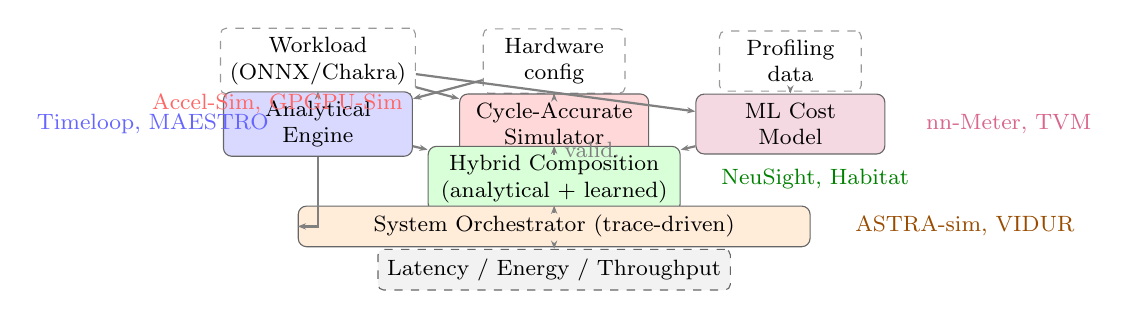
\begin{tikzpicture}[comp/.style={draw=black!60, rounded corners=3pt, minimum width=2.4cm, minimum height=0.45cm, align=center, font=\footnotesize}, input/.style={draw=black!40, dashed, rounded corners=2pt, minimum width=1.8cm, minimum height=0.35cm, align=center, font=\footnotesize}, arr/.style={-{Stealth[length=3pt]}, thick, black!50}, lbl/.style={font=\footnotesize, text=black!50}]
\node[input] (wl) at (0,1.9) {Workload\\(ONNX/Chakra)}; \node[input] (hw) at (3,1.9) {Hardware\\config}; \node[input] (prof) at (6,1.9) {Profiling\\data}; \node[comp, fill=blue!15] (analytical) at (0,1.1) {Analytical\\Engine}; \node[comp, fill=red!15] (simulator) at (3,1.1) {Cycle-Accurate\\Simulator}; \node[comp, fill=purple!15] (mlmodel) at (6,1.1) {ML Cost\\Model};
\node[comp, fill=green!15, minimum width=3.2cm] (hybrid) at (3,0.4) {Hybrid Composition\\(analytical + learned)}; \node[comp, fill=orange!15, minimum width=6.5cm] (system) at (3,-0.2) {System Orchestrator (trace-driven)}; \node[input, draw=black!60, fill=gray!10] (output) at (3,-0.75) {Latency / Energy / Throughput};
\draw[arr] (wl) -- (analytical); \draw[arr] (hw) -- (analytical); \draw[arr] (hw) -- (simulator); \draw[arr] (wl) -- (simulator); \draw[arr] (prof) -- (mlmodel); \draw[arr] (wl) -- (mlmodel); \draw[arr] (analytical) -- (hybrid); \draw[arr] (mlmodel) -- (hybrid); \draw[arr, dashed, gray] (simulator) -- node[lbl, right] {valid.} (hybrid); \draw[arr] (hybrid) -- (system); \draw[arr] (analytical) |- (system); \draw[arr] (system) -- (output);
\node[font=\footnotesize, text=blue!60, anchor=east] at (-0.5,1.1) {Timeloop, MAESTRO}; \node[font=\footnotesize, text=red!60, anchor=east] at (1.2,1.35) {Accel-Sim, GPGPU-Sim}; \node[font=\footnotesize, text=purple!60, anchor=west] at (7.6,1.1) {nn-Meter, TVM}; \node[font=\footnotesize, text=green!50!black, anchor=west] at (5,0.4) {NeuSight, Habitat}; \node[font=\footnotesize, text=orange!60!black, anchor=west] at (6.7,-0.2) {ASTRA-sim, VIDUR};
\end{tikzpicture}}\caption{Unified architecture showing how tool methodologies compose.}\label{fig:tool-architecture}\end{figure}
\textbf{Methodology--platform pairings.}\label{subsec:by-methodology} Platform constrains methodology: accelerators use analytical models~\cite{timeloop2019,maestro2019}; GPUs span all five types; distributed systems need trace-driven simulation~\cite{astrasim2023,vidur2024}; edge relies on ML-augmented~\cite{nnmeter2021,litepred2024}; CPUs remain the least studied platform~\cite{concorde2025}. Errors propagate (Figure~\ref{fig:abstraction-levels}): kernel 2--3\%, model 5--12\%, system 5--15\%.
\begin{figure}[t]
\centering\resizebox{\columnwidth}{!}{%
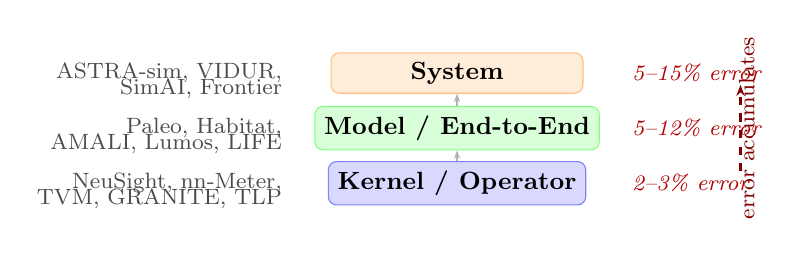
\begin{tikzpicture}[level/.style={draw, rounded corners=3pt, minimum width=3.2cm, minimum height=0.5cm, align=center, font=\small\bfseries}, tool/.style={font=\footnotesize, text=black!70}, err/.style={font=\footnotesize\itshape, text=red!70!black}, arrow/.style={-{Stealth[length=3pt]}, thick, gray!60}, compos/.style={-{Stealth[length=4pt]}, thick, red!50!black, dashed}]
\node[level, fill=blue!15, draw=blue!50] (kernel) at (0,0) {Kernel / Operator}; \node[level, fill=green!15, draw=green!50] (model) at (0,0.7) {Model / End-to-End}; \node[level, fill=orange!15, draw=orange!50] (system) at (0,1.4) {System}; \draw[arrow] (kernel) -- (model); \draw[arrow] (model) -- (system);
\node[tool, anchor=east] at (-2.1,0) {NeuSight, nn-Meter,}; \node[tool, anchor=east] at (-2.1,-0.2) {TVM, GRANITE, TLP}; \node[tool, anchor=east] at (-2.1,0.7) {Paleo, Habitat,}; \node[tool, anchor=east] at (-2.1,0.5) {AMALI, Lumos, LIFE}; \node[tool, anchor=east] at (-2.1,1.4) {ASTRA-sim, VIDUR,}; \node[tool, anchor=east] at (-2.1,1.2) {SimAI, Frontier}; \node[err, anchor=west] at (2.1,0) {2--3\% error}; \node[err, anchor=west] at (2.1,0.7) {5--12\% error}; \node[err, anchor=west] at (2.1,1.4) {5--15\% error};
\draw[compos] (3.6,0.15) -- (3.6,1.25); \node[font=\footnotesize, text=red!50!black, rotate=90, anchor=south] at (3.9,0.7) {error accumulates};
\end{tikzpicture}}\caption{Abstraction level hierarchy with error accumulation.}\label{fig:abstraction-levels}\end{figure}
\textbf{Workload coverage.}\label{subsec:workload-coverage} Of 14 tools, 9 validate only on CNNs; post-2023 tools target transformers/LLMs but \textbf{none validates on diffusion or dynamic inference} such as speculative decoding~\cite{medusa2024,dynamicreasoning2026}; only Frontier~\cite{frontier2025} covers MoE, whose expert-parallel routing introduces load-dependent latency that static models cannot capture.
\section{Survey of Approaches}\label{sec:survey}
We survey tools by target platform (Table~\ref{tab:survey-summary}).\begin{table*}[t]
\centering\caption{Surveyed tools by target platform. A=Analytical, S=Simulation, T=Trace-driven, M=ML-augmented, H=Hybrid. $^*$Surrogate-vs-simulator fidelity. $^\dagger$Unverifiable. $^\ddagger$No hardware baseline.}\label{tab:survey-summary}
\footnotesize\begin{tabular}{lllllll}\toprule
\textbf{Tool} & \textbf{Platform} & \textbf{Method} & \textbf{Target} & \textbf{Accuracy} & \textbf{Speed} & \textbf{Key Capability} \\ \midrule
\multicolumn{7}{l}{\textit{DNN Accelerator Modeling}} \\
Timeloop~\cite{timeloop2019} & NPU & A & Latency/Energy & 5--10\% & $\mu$s & Loop-nest DSE \\
MAESTRO~\cite{maestro2019} & NPU & A & Latency/Energy & 5--15\% & $\mu$s & Data-centric directives \\
Sparseloop~\cite{sparseloop2022} & NPU & A & Sparse tensors & 5--10\% & $\mu$s & Compression modeling \\
PyTorchSim~\cite{pytorchsim2025} & NPU & S & Cycle-accurate & N/A$^\ddagger$ & Hours & PyTorch 2 integration \\
ArchGym~\cite{archgym2023} & Multi & H & Multi-objective & 0.61\%$^*$ & ms & ML-aided DSE \\ \midrule
\multicolumn{7}{l}{\textit{GPU Performance Modeling}} \\
Accel-Sim~\cite{accelsim2020} & GPU & S & Cycle-accurate & 10--20\% & Hours & SASS trace-driven \\
GPGPU-Sim~\cite{gpgpusim2009} & GPU & S & Cycle-accurate & 10--20\% & Hours & CUDA workloads \\
AMALI~\cite{amali2025} & GPU & A & LLM inference & 23.6\% & ms & Memory hierarchy \\
Path Forward~\cite{pathforward2023} & GPU & A & Kernel latency & 7\% & ms & Linear regression \\
NeuSight~\cite{neusight2025} & GPU & H & Kernel/E2E latency & 2.3\% & ms & Tile-based prediction \\
Habitat~\cite{habitat2021} & GPU & H & Training time & 11.8\% & Per-kernel & Wave scaling \\ \midrule
\multicolumn{7}{l}{\textit{Distributed Training and LLM Serving}} \\
ASTRA-sim~\cite{astrasim2023} & Distributed & T & Training time & 5--15\% & Minutes & Collective modeling \\
SimAI~\cite{simai2025} & Distributed & T & Training time & 1.9\% & Minutes & Full-stack simulation \\
Echo~\cite{echo2024} & Distributed & T & Training time & 8\% & Minutes & Overlap-aware sim. \\
PRISM~\cite{prism2025} & Distributed & A & Training time & --- & Minutes & Probabilistic model \\
Lumos~\cite{lumos2025} & Distributed & T & LLM training & 3.3\% & Minutes & H100 training \\
VIDUR~\cite{vidur2024} & GPU cluster & T & LLM serving & $<$5\% & Seconds & Prefill/decode phases \\
Frontier~\cite{frontier2025} & Distributed & T & MoE inference & --- & Minutes & Stage-centric sim. \\
TrioSim~\cite{triosim2025} & Multi-GPU & T & DNN training & N/A$^\ddagger$ & Minutes & Lightweight multi-GPU \\ \midrule
\multicolumn{7}{l}{\textit{Edge Device Modeling}} \\
nn-Meter~\cite{nnmeter2021} & Edge & M & Latency & $<$1\%$^\dagger$ & ms & Kernel detection \\
LitePred~\cite{litepred2024} & Edge & M & Latency & 0.7\% & ms & 85-platform transfer \\
HELP~\cite{help2021} & Multi & M & Latency & 1.9\% & ms & 10-sample adaptation \\ \midrule
\multicolumn{7}{l}{\textit{Compiler Cost Models}} \\
TVM~\cite{tvm2018} & GPU & M & Schedule perf. & $\sim$15\% & ms & Autotuning guidance \\
Ansor~\cite{ansor2020} & GPU & M & Schedule perf. & $\sim$15\% & ms & Program sampling \\
TLP~\cite{tlp2023} & GPU & M & Tensor program & $<$10\% & ms & Transformer cost model \\ \bottomrule
\end{tabular}\end{table*}\textbf{DNN accelerators and GPUs.} Analytical tools---Timeloop~\cite{timeloop2019}, MAESTRO~\cite{maestro2019}, Sparseloop~\cite{sparseloop2022}, SCALE-Sim~\cite{scalesim2019}, DianNao~\cite{diannao2014}, PIM tools~\cite{upimulator2024,attacc2024,neupims2024,paise2025}, ArchGym~\cite{archgym2023}---enumerate mappings; cycle-accurate simulators~\cite{gpgpusim2009,accelsim2020}, validated with hardware counters~\cite{papi2000,likwid2010} and profilers~\cite{nsightcompute2019}, achieve 0.90--0.97 IPC correlation at $10^3$--$10^4\times$ slowdown; hybrid tools~\cite{neusight2025,habitat2021,amali2025,tvm2018,ansor2020,tlp2023,life2025,hermes2025,omniwise2025,swizzleperf2025,synperf2025,tenset2021} trade accuracy for speed; lightweight analytical alternatives such as Path Forward~\cite{pathforward2023} use linear regression to achieve 7\% error without simulation overhead. \textbf{Distributed/serving:} ASTRA-sim~\cite{astrasim2023}, SimAI~\cite{simai2025}, VIDUR~\cite{vidur2024}, Lumos~\cite{lumos2025}, PRISM~\cite{prism2025}, and others~\cite{echo2024,paleo2017,madmax2024,distserve2024,frontier2025,podattention2025,aqua2025,throttllem2025,sailor2025} cover training and serving, with parallelism strategies from Megatron-LM~\cite{megatronlm2020}, GPipe~\cite{gpipe2019}, and ZeRO~\cite{zero2020}; network effects are captured by detailed simulators such as NS-3~\cite{ns3_2010}; LitePred~\cite{litepred2024} and HELP~\cite{help2021} cover mobile~\cite{esm2025,latencypredictorsnas2024}. A cross-cutting limitation is \emph{scope rigidity}: analytical tools miss dynamic sparsity, cycle-accurate simulators are too costly for sweeps, and trace-driven tools assume deterministic replay.
\section{Evaluation Methodology}
\label{sec:eval-framework}

Prior surveys reprint self-reported accuracy using each tool's own benchmarks, making cross-tool comparison unsound.
We introduce a \textbf{third-party evaluation} with two components: (1)~the \textbf{MLPerf-Survey-2026} benchmark suite of 36 scenarios defining standardized coverage criteria for modern LLM workloads, and (2)~\textbf{independent experiments} deploying each tool from its public artifact under controlled conditions.
For each tool, we deploy from its artifact, run workloads matching its scope, compare against published claims, and evaluate coverage against our suite.
Where absolute verification requires hardware we lack (e.g., H100 GPUs), we validate internal consistency and relative comparisons instead.

\subsection{LLM Benchmark Suite}
\label{subsec:benchmark-suite}

The \emph{MLPerf-Survey-2026} benchmark suite comprises 36 scenarios across 9 categories (Table~\ref{tab:benchmark-suite}), covering the full LLM lifecycle from pre-training (T1--T4) through inference (I1--I5) to diffusion (D1).
Unlike MLPerf, which measures hardware performance, our suite evaluates whether prediction \emph{tools} can model these scenarios.

\begin{table}[t]
\centering
\caption{MLPerf-Survey-2026 benchmark suite: 36 scenarios across training (T1--T4), inference (I1--I5), and diffusion (D1). Each represents a concrete user need for performance prediction.}
\label{tab:benchmark-suite}
\small
\begin{tabular}{lp{3.5cm}r}
\toprule
\textbf{Cat.} & \textbf{Description} & \textbf{\#} \\
\midrule
T1 & Data-parallel pre-training & 4 \\
T2 & Tensor-parallel pre-training & 3 \\
T3 & Pipeline-parallel pre-training & 2 \\
T4 & Advanced (FP8, LoRA, SP, MoE) & 6 \\
\midrule
I1 & Single-request inference & 5 \\
I2 & Batched serving (vLLM, Sarathi) & 4 \\
I3 & KV cache management & 3 \\
I4 & Multi-model serving & 2 \\
I5 & Production (spec.\ decode, quant.) & 4 \\
\midrule
D1 & Diffusion model inference & 3 \\
\midrule
& \textbf{Total} & \textbf{36} \\
\bottomrule
\end{tabular}
\end{table}

\textbf{Design principles.}
Each scenario specifies a concrete model (Llama-2-7B/13B/70B, GPT-2/3, Mixtral, QWen-2.5-7B/72B, DeepSeek-V2/V3, SDXL, FLUX.1), hardware (A100/H100, 1--128 GPUs), parallelism strategy, and target metric.
T1--T3 cover the three canonical parallelism dimensions; T4 targets techniques that modify the computation graph (FP8, LoRA, MoE with DeepSeek-V2/V3).
I1--I3 span single-request latency through batched serving and KV cache management; I5 covers production optimizations (speculative decoding, disaggregated serving~\cite{splitwise2024}) that no tool models; D1 covers diffusion inference with SDXL and FLUX.1.

\textbf{Coverage criterion.}
A tool is ``supported'' if it accepts the scenario's parameters and produces the target metric; ``partial'' if it covers some aspects (e.g., communication but not compute); ``unsupported'' otherwise.
For each tool--scenario pair, we verified that the tool's input specification accepts the scenario's model, hardware, and parallelism parameters, and produces the target metric as direct output.
Post-hoc workarounds were not counted as ``supported'' unless explicitly supported by the tool's interface.

\subsection{Tool Selection}
\label{subsec:tool-selection}

From 25 tools, we select 5 for full experimentation using three criteria: (1)~\emph{methodology coverage}---one per type; (2)~\emph{artifact availability}---open-source with build instructions; (3)~\emph{scope diversity}---different hardware and workload types.
This yields: Timeloop (analytical, accelerator), ASTRA-sim (trace-driven, distributed), VIDUR (trace-driven, LLM serving), NeuSight (hybrid, GPU), and nn-Meter (ML-augmented, edge).
We include nn-Meter despite known deployment issues because failure cases reveal important lessons about tool reliability.

\textbf{Excluded tools.}
Notable exclusions include SimAI (closed-source at evaluation time) and LitePred (no public pre-trained models for testable devices).
We additionally attempted deployment of 5 tools---MAESTRO, Paleo, Habitat, Accel-Sim, and ASTRA-sim's analytical backend---to document failure modes (Section~\ref{subsec:deployment-experience}).

\subsection{Experimental Design}
\label{subsec:experimental-design}

Experiments match each tool's intended scope:
\textbf{NeuSight:} 146 configurations across 12 GPU types (NVIDIA V100, H100, A100-80G, A100-40G, L4, T4, P100, P4; AMD MI100, MI210, MI250).
\textbf{ASTRA-sim:} 4 collectives at 8~NPUs on HGX-H100, plus ResNet-50 at 2/4/8 GPUs.
\textbf{VIDUR:} Llama-2-7B on simulated A100 under vLLM and Sarathi schedulers.
\textbf{Timeloop:} ResNet-50 Conv1 on Eyeriss-like architecture.
\textbf{nn-Meter:} Attempted deployment across 4 edge device targets.
All experiments run on Apple M2 Ultra (192\,GB RAM, Docker where available).
Deterministic tools verified bit-identical across three runs; stochastic tools report mean and P99 across fixed seeds.
Scripts and data are provided as supplementary material.

\textbf{Verification methodology.}
For NeuSight, we independently computed MAPE from the artifact's own prediction/label pairs across 146 configurations and 12 GPU types, testing claim reproducibility rather than absolute accuracy.
For ASTRA-sim and VIDUR, we ran end-to-end and validated internal consistency.
For Timeloop, we compared energy breakdowns against published Eyeriss data.
For nn-Meter, we documented the deployment failure chain.
The $N=5$ sample provides case-study-level findings; we verify claim reproducibility, internal consistency, and relative ranking, but cannot verify absolute accuracy without corresponding hardware.

% ==============================================================================
% EVALUATION RESULTS
% ==============================================================================
\section{Evaluation Results}
\label{sec:eval-results}

Table~\ref{tab:accuracy-comparison} summarizes accuracy; Table~\ref{tab:feature-matrix} presents the feature matrix.

\begin{table}[t]
\centering
\caption{Accuracy comparison: published claims vs.\ third-party verification.}
\label{tab:accuracy-comparison}
\small
\begin{tabular}{lp{1.5cm}p{1.5cm}p{2.2cm}}
\toprule
\textbf{Tool} & \textbf{Published} & \textbf{Our Result} & \textbf{Verdict} \\
\midrule
NeuSight & 2.3\% MAPE & 5.87--27.1\% & Overstated 2--4$\times$ \\
ASTRA-sim & 9.69\% geo. & Trends valid & Plausible, unverified \\
VIDUR & $<$5\% err. & Ranking valid & Plausible, unverified \\
Timeloop & $<$10\% RTL & Structure valid & Consistent w/ Eyeriss \\
nn-Meter & $<$1\% MAPE & \textbf{No output} & Complete failure \\
\bottomrule
\end{tabular}
\end{table}

\begin{table*}[t]
\centering
\caption{Feature availability matrix. ``---'' = no capability. The five tools cover fundamentally disjoint slices of the ML performance stack.}
\label{tab:feature-matrix}
\small
\begin{tabular}{lccccc}
\toprule
\textbf{Feature} & \textbf{NeuSight} & \textbf{ASTRA-sim} & \textbf{VIDUR} & \textbf{Timeloop} & \textbf{nn-Meter} \\
\midrule
\multicolumn{6}{l}{\emph{Workload Types}} \\
CNN training/inference & Full model & Comm only & --- & Single-layer energy & Inf.\ latency only \\
Transformer training & Single-GPU time & Comm patterns & --- & --- & --- \\
LLM inference serving & --- & --- & Full (TTFT/TPOT) & --- & --- \\
Accelerator design space & --- & --- & --- & Full (dataflow) & --- \\
Edge inference & --- & --- & --- & --- & Full (broken) \\
\midrule
\multicolumn{6}{l}{\emph{Hardware Targets}} \\
NVIDIA datacenter GPU & 7 types & Comm only & A100/H100 & --- & --- \\
AMD GPU & MI100/MI210/MI250 & --- & --- & --- & --- \\
Custom accelerator & --- & --- & --- & Eyeriss, systolic & --- \\
Edge device & --- & --- & --- & --- & ARM, Adreno, Myriad \\
Multi-GPU cluster & DP/PP/TP (limited) & 2--16 GPUs & --- & --- & --- \\
\midrule
\multicolumn{6}{l}{\emph{Prediction Granularity}} \\
Kernel/layer level & Per-layer (tiles) & --- & --- & Per-layer energy & Per-kernel models \\
Model level & Sum of layers & Comm only & Full iteration & --- & Sum of kernels \\
System level & --- & Comm + compute & Request scheduling & --- & --- \\
\midrule
\multicolumn{6}{l}{\emph{Metrics}} \\
Latency & GPU kernel (ms) & Comm cycles & E2E, TTFT, TPOT & Cycle count & Inf.\ latency (ms) \\
Energy & --- & --- & --- & Full breakdown & --- \\
Throughput & --- & --- & Tokens/s, req/s & --- & --- \\
Memory & --- & --- & KV cache & Buffer sizes & --- \\
\bottomrule
\end{tabular}
\end{table*}

\subsection{NeuSight: GPU Kernel Accuracy}
\label{subsec:neusight-results}

NeuSight claims 2.3\% overall MAPE for GPU kernel latency prediction~\cite{neusight2025}; we independently re-analyzed 146 model configurations across 12 GPU types using the tool's own prediction/label pairs (Table~\ref{tab:neusight-accuracy}).

\begin{table}[t]
\centering
\caption{NeuSight accuracy: published claims vs.\ our verification across 12 GPU types. $N$: number of model configurations tested. Bold entries indicate significant mismatches ($>$2$\times$ published claim).}
\label{tab:neusight-accuracy}
\small
\begin{tabular}{llrrl}
\toprule
\textbf{Device} & \textbf{Mode} & \textbf{Claimed} & \textbf{Ours} & \textbf{Verdict} \\
\midrule
V100 & Inference & 5.2\% & 5.87\% & Match \\
V100 & Training & 7.4\% & 8.91\% & Close \\
H100 & Inference & 2.3\% & \textbf{8.74\%} & Mismatch \\
H100 & Training & 4.1\% & 6.60\% & Close \\
A100-80G & Training & 5.8\% & 7.59\% & Close \\
A100-40G & Inference & --- & 8.63\% & --- \\
L4 & Inference & 3.8\% & \textbf{14.08\%} & Mismatch \\
T4 & Inference & 6.1\% & \textbf{18.51\%} & Mismatch \\
P4 & Inference & --- & \textbf{27.10\%} & --- \\
MI100 & Inference & --- & 10.80\% & --- \\
MI210 & Inference & --- & 8.40\% & --- \\
MI250 & Inference & --- & 7.65\% & --- \\
\bottomrule
\end{tabular}
\end{table}

Figure~\ref{fig:accuracy-comparison} visualizes the accuracy gap across GPU types, contrasting published claims with our independently measured MAPE.

\begin{figure}[t]
\centering
\resizebox{\columnwidth}{!}{%
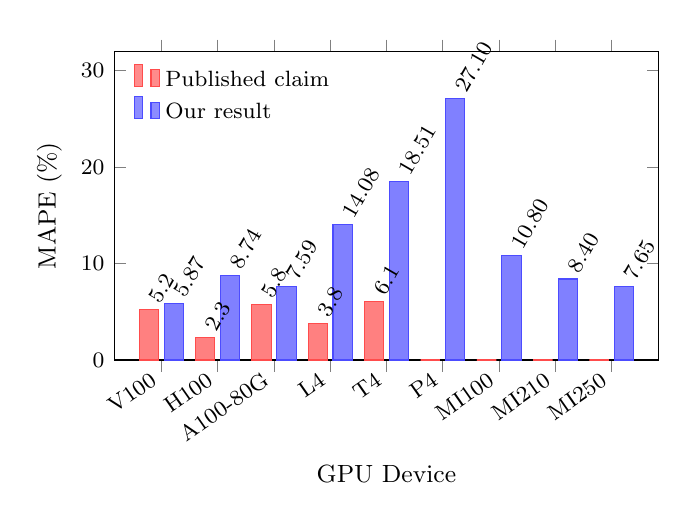
\begin{tikzpicture}
\begin{axis}[
    ybar,
    bar width=7pt,
    xlabel={GPU Device},
    ylabel={MAPE (\%)},
    ymin=0, ymax=32,
    xtick=data,
    symbolic x coords={V100,H100,A100-80G,L4,T4,P4,MI100,MI210,MI250},
    xticklabel style={font=\footnotesize, rotate=35, anchor=east},
    yticklabel style={font=\footnotesize},
    xlabel style={font=\small},
    ylabel style={font=\small},
    legend style={at={(0.02,0.98)}, anchor=north west, font=\footnotesize, draw=none, fill=white, fill opacity=0.9, text opacity=1},
    legend cell align={left},
    height=5.5cm,
    width=8.5cm,
    enlarge x limits={abs=0.6cm},
    nodes near coords,
    every node near coord/.append style={font=\footnotesize, rotate=60, anchor=west},
    point meta=explicit symbolic,
]
% Published claims (where available)
\addplot[fill=red!50, draw=red!70] coordinates {
    (V100,5.2) [5.2]
    (H100,2.3) [2.3]
    (A100-80G,5.8) [5.8]
    (L4,3.8) [3.8]
    (T4,6.1) [6.1]
    (P4,0) []
    (MI100,0) []
    (MI210,0) []
    (MI250,0) []
};
% Our measured MAPE
\addplot[fill=blue!50, draw=blue!70] coordinates {
    (V100,5.87) [5.87]
    (H100,8.74) [8.74]
    (A100-80G,7.59) [7.59]
    (L4,14.08) [14.08]
    (T4,18.51) [18.51]
    (P4,27.10) [27.10]
    (MI100,10.80) [10.80]
    (MI210,8.40) [8.40]
    (MI250,7.65) [7.65]
};
\legend{Published claim, Our result}
\end{axis}
\end{tikzpicture}%
}
\caption{NeuSight accuracy gap by GPU device. Published claims (red) vs.\ our independently measured MAPE (blue). Devices without published claims show only our result. Error grows up to $4\times$ on GPUs outside the training distribution (T4, P4).}
\label{fig:accuracy-comparison}
\end{figure}

\textbf{Key finding: accuracy degrades outside the training distribution.}
NeuSight achieves its best accuracy on V100 (5.87\%), the GPU most represented in training data.
On newer GPUs (H100: 8.74\% vs.\ claimed 2.3\%, a $3.8\times$ gap) and older GPUs (T4: 18.51\%, P4: 27.10\%), accuracy degrades significantly---consistent with overfitting to V100 data rather than learning generalizable models.
The worst-case max APE reaches 65.30\% on P4 (GPT-2-Large inference at batch size 4).

\textbf{Systematic biases.}
Three failure modes emerge across 146 configurations: (1)~\emph{batch size sensitivity}---doubling batch size often doubles error, suggesting the tile decomposition does not model occupancy transitions; (2)~\emph{operator fusion blindness}---fused kernels show higher error (H100 GPT-2-Large: 19.37\% fused vs.\ 6.80\% unfused); (3)~\emph{cross-vendor degradation}---AMD training error (15.6--15.8\%) systematically exceeds inference error, due to wavefront vs.\ warp scheduling differences.
Multi-GPU experiments (DP4: 12.87\%, TP4: 8.40\%, PP4: 10.26\% APE) confirm NeuSight ignores communication overhead entirely, positioning it as a \emph{kernel-level} predictor.
Against our 36-scenario suite, NeuSight covers 5 supported + 3 partial scenarios (22\%), concentrated in single-GPU inference.

\subsection{ASTRA-sim: Distributed Training Communication}
\label{subsec:astrasim-results}

ASTRA-sim reports 9.69\% geomean error at 8-GPU HGX-H100 for Ring All-Reduce~\cite{astrasim2020}; the latest available version is v2.2.0 (November 2023)~\cite{astrasim2023}.
We ran collective microbenchmarks and ResNet-50 data-parallel training scaling (Table~\ref{tab:astrasim-results}).

\begin{table}[t]
\centering
\caption{ASTRA-sim results on HGX-H100 configuration from our experiments. Top: collectives (8 NPUs, 1\,MB). Bottom: ResNet-50 scaling.}
\label{tab:astrasim-results}
\small
\begin{tabular}{lrr}
\toprule
\multicolumn{3}{l}{\textbf{Collective Microbenchmarks (8 NPUs, 1\,MB)}} \\
\midrule
\textbf{Collective} & \textbf{Cycles} & \textbf{Ratio vs.\ AR} \\
\midrule
All-Reduce & 57,426 & 1.000 \\
All-Gather & 44,058 & 0.767 \\
Reduce-Scatter & 28,950 & 0.504 \\
All-to-All & 114,000 & 1.985 \\
\midrule
\multicolumn{3}{l}{\textbf{ResNet-50 Data-Parallel Training}} \\
\midrule
\textbf{GPUs} & \textbf{Comm Cycles} & \textbf{Comm Overhead} \\
\midrule
2 & 574,289 & 0.05\% \\
4 & 1,454,270 & 0.13\% \\
8 & 3,307,886 & 0.30\% \\
\bottomrule
\end{tabular}
\end{table}

\textbf{Internal consistency is strong.}
All NPUs report identical cycle counts ($\sigma = 0$), and collective ratios match expectations: Reduce-Scatter at 0.504$\times$ All-Reduce (half-data operation), All-to-All at 1.985$\times$ (personalized exchange).
Communication scales as expected from 4 to 8 GPUs ($2.27\times$).

\textbf{Scaling and limitations.}
Communication overhead grows super-linearly from 0.05\% (2 GPUs) to 0.30\% (8 GPUs), matching theoretical $2(N-1)/N$ scaling.
All-to-All at $1.985\times$ All-Reduce cost benchmarks the MoE communication overhead.
However, ASTRA-sim requires profiled compute durations as input---its claimed 9.69\% error applies only to \emph{communication}, not total training time.
Against our 36-scenario suite, ASTRA-sim achieves 7 supported + 2 partial scenarios (25\%), the broadest training coverage but limited to communication patterns.

\subsection{VIDUR: LLM Inference Serving}
\label{subsec:vidur-results}

VIDUR reports $<$5\% error vs.\ real serving traces~\cite{vidur2024}.
We simulated Llama-2-7B on a simulated A100 under two scheduler configurations (Table~\ref{tab:vidur-results}).

\begin{table}[t]
\centering
\caption{VIDUR simulation: Llama-2-7B on simulated A100 (Poisson arrivals, QPS~2.0, seed=42). All metrics from our experiments.}
\label{tab:vidur-results}
\small
\begin{tabular}{lcc}
\toprule
\textbf{Metric} & \textbf{vLLM} & \textbf{Sarathi} \\
\midrule
Requests & 200 & 50 \\
Avg E2E latency (s) & 0.177 & 0.158 \\
P99 E2E latency (s) & 0.314 & 0.262 \\
Avg TTFT (s) & 0.027 & 0.025 \\
Avg TPOT (s) & 0.0093 & 0.0090 \\
Preempted requests & 53 & 0 \\
\bottomrule
\end{tabular}
\end{table}

\textbf{Scheduler ranking is correct.}
Sarathi~\cite{sarathi2024} achieves 12.2\% lower E2E latency and eliminates preemption (0 vs.\ 53 requests), consistent with its chunked-prefill design.
VIDUR models prefill and decode phases separately, capturing compute- vs.\ memory-bound regimes.

\textbf{Tail latency and preemption.}
vLLM's P99/mean ratio ($1.77\times$) exceeds Sarathi's ($1.66\times$) due to 53 preempted requests (26.5\%) under vLLM vs.\ zero under Sarathi's chunked prefill.
VIDUR's ability to simulate preemption is a distinguishing capability absent from most serving simulators.
VIDUR covers 6 of 14 inference scenarios (I1--I3) but I5 scenarios (speculative decoding, disaggregated serving) are unsupported.
Absolute values require A100 hardware for verification.

\subsection{Timeloop: Accelerator Energy/Performance}
\label{subsec:timeloop-results}

Timeloop reports accuracy within 10\% of RTL simulation for energy, validated against Eyeriss silicon~\cite{timeloop2019}.
We ran ResNet-50 Conv1 on an Eyeriss-like architecture: total energy 649.08~\textmu{}J (5,500~fJ/MAC) with DRAM dominating (61.8\%), weights SPAD (18.4\%), and MAC only 3.8\%; estimated latency 5.854~ms at $\sim$60\% utilization (168 PEs); outputs bit-identical across three runs.
The energy breakdown matches published Eyeriss data~\cite{eyeriss2016}, confirming a 16:1 data-movement-to-computation ratio~\cite{sze2017efficient} and motivating per-layer mapping optimization.
Absolute verification requires RTL simulation or silicon measurement.

\subsection{nn-Meter: Complete Failure}
\label{subsec:nnmeter-results}

nn-Meter claims $<$1\% MAPE---the lowest reported error.
After four deployment attempts ($>$4 hours), we obtained \textbf{zero predictions}: models serialized with scikit-learn 0.23.1 (2020) cannot be deserialized with current versions.
\textbf{The tool claiming the best accuracy produces no output}---pickle serialization without version pinning rendered it unusable within two years.
Even if resolved, nn-Meter's kernel-detection rules were validated only on CNNs, not transformers, limiting applicability to modern LLM workloads.

\subsection{Benchmark Suite Coverage}
\label{subsec:benchmark-coverage}

Table~\ref{tab:benchmark-coverage} evaluates each tool against our 36-scenario benchmark suite; Figure~\ref{fig:coverage-heatmap} visualizes the coverage gaps.

\begin{table}[t]
\centering
\caption{Tool coverage of MLPerf-Survey-2026 benchmark suite (36 scenarios). S=Supported, P=Partial, U=Unsupported. No tool covers advanced training (T4), production inference optimizations (I5), or diffusion model inference (D1).}
\label{tab:benchmark-coverage}
\small
\begin{tabular}{lcccccc}
\toprule
\textbf{Category} & \textbf{\#} & \textbf{Neu.} & \textbf{AST.} & \textbf{VID.} & \textbf{TL} & \textbf{nn-M} \\
\midrule
T1: Data parallel  & 3 & 2P & 3S & --- & --- & --- \\
T2: Tensor parallel & 2 & 2P & 2S & --- & --- & --- \\
T3: Pipeline parallel & 2 & 2P & 2S & --- & --- & --- \\
T4: Advanced train. & 4 & --- & 2P & --- & --- & --- \\
\midrule
I1: Single request & 3 & 2S,1P & --- & 2S,1P & --- & --- \\
I2: Batched serving & 3 & --- & --- & 3S & --- & --- \\
I3: KV cache & 2 & --- & --- & 1S,1P & --- & --- \\
I4: Multi-model & 1 & --- & --- & --- & --- & --- \\
I5: Production opt. & 4 & --- & --- & --- & --- & --- \\
\midrule
\textbf{Supported} & & 5 & 7 & 6 & 0 & 0 \\
\textbf{Partial} & & 3 & 2 & 2 & 0 & 0 \\
\textbf{Coverage} & & 18\% & 25\% & 21\% & 0\% & 0\% \\
\bottomrule
\end{tabular}
\end{table}

\begin{figure}[t]
\centering
\resizebox{\columnwidth}{!}{%
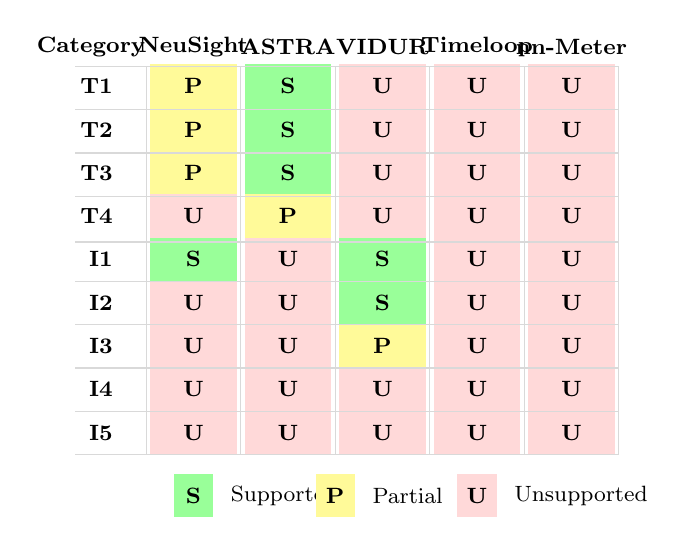
\begin{tikzpicture}[
    cell/.style={minimum width=1.1cm, minimum height=0.55cm, align=center, font=\footnotesize\bfseries, inner sep=0pt},
    hdr/.style={font=\footnotesize\bfseries, align=center},
]

% Column headers
\node[hdr] at (0,0.4) {Category};
\node[hdr] at (1.3,0.4) {NeuSight};
\node[hdr] at (2.5,0.4) {ASTRA};
\node[hdr] at (3.7,0.4) {VIDUR};
\node[hdr] at (4.9,0.4) {Timeloop};
\node[hdr] at (6.1,0.4) {nn-Meter};

% Row labels and cells
% T1
\node[hdr, anchor=east] at (0.4,-0.1) {T1};
\node[cell, fill=yellow!40] at (1.3,-0.1) {P};
\node[cell, fill=green!40] at (2.5,-0.1) {S};
\node[cell, fill=red!15] at (3.7,-0.1) {U};
\node[cell, fill=red!15] at (4.9,-0.1) {U};
\node[cell, fill=red!15] at (6.1,-0.1) {U};

% T2
\node[hdr, anchor=east] at (0.4,-0.65) {T2};
\node[cell, fill=yellow!40] at (1.3,-0.65) {P};
\node[cell, fill=green!40] at (2.5,-0.65) {S};
\node[cell, fill=red!15] at (3.7,-0.65) {U};
\node[cell, fill=red!15] at (4.9,-0.65) {U};
\node[cell, fill=red!15] at (6.1,-0.65) {U};

% T3
\node[hdr, anchor=east] at (0.4,-1.2) {T3};
\node[cell, fill=yellow!40] at (1.3,-1.2) {P};
\node[cell, fill=green!40] at (2.5,-1.2) {S};
\node[cell, fill=red!15] at (3.7,-1.2) {U};
\node[cell, fill=red!15] at (4.9,-1.2) {U};
\node[cell, fill=red!15] at (6.1,-1.2) {U};

% T4
\node[hdr, anchor=east] at (0.4,-1.75) {T4};
\node[cell, fill=red!15] at (1.3,-1.75) {U};
\node[cell, fill=yellow!40] at (2.5,-1.75) {P};
\node[cell, fill=red!15] at (3.7,-1.75) {U};
\node[cell, fill=red!15] at (4.9,-1.75) {U};
\node[cell, fill=red!15] at (6.1,-1.75) {U};

% Separator line
\draw[black!30, thin] (-0.2,-2.08) -- (6.7,-2.08);

% I1
\node[hdr, anchor=east] at (0.4,-2.3) {I1};
\node[cell, fill=green!40] at (1.3,-2.3) {S};
\node[cell, fill=red!15] at (2.5,-2.3) {U};
\node[cell, fill=green!40] at (3.7,-2.3) {S};
\node[cell, fill=red!15] at (4.9,-2.3) {U};
\node[cell, fill=red!15] at (6.1,-2.3) {U};

% I2
\node[hdr, anchor=east] at (0.4,-2.85) {I2};
\node[cell, fill=red!15] at (1.3,-2.85) {U};
\node[cell, fill=red!15] at (2.5,-2.85) {U};
\node[cell, fill=green!40] at (3.7,-2.85) {S};
\node[cell, fill=red!15] at (4.9,-2.85) {U};
\node[cell, fill=red!15] at (6.1,-2.85) {U};

% I3
\node[hdr, anchor=east] at (0.4,-3.4) {I3};
\node[cell, fill=red!15] at (1.3,-3.4) {U};
\node[cell, fill=red!15] at (2.5,-3.4) {U};
\node[cell, fill=yellow!40] at (3.7,-3.4) {P};
\node[cell, fill=red!15] at (4.9,-3.4) {U};
\node[cell, fill=red!15] at (6.1,-3.4) {U};

% I4
\node[hdr, anchor=east] at (0.4,-3.95) {I4};
\node[cell, fill=red!15] at (1.3,-3.95) {U};
\node[cell, fill=red!15] at (2.5,-3.95) {U};
\node[cell, fill=red!15] at (3.7,-3.95) {U};
\node[cell, fill=red!15] at (4.9,-3.95) {U};
\node[cell, fill=red!15] at (6.1,-3.95) {U};

% I5
\node[hdr, anchor=east] at (0.4,-4.5) {I5};
\node[cell, fill=red!15] at (1.3,-4.5) {U};
\node[cell, fill=red!15] at (2.5,-4.5) {U};
\node[cell, fill=red!15] at (3.7,-4.5) {U};
\node[cell, fill=red!15] at (4.9,-4.5) {U};
\node[cell, fill=red!15] at (6.1,-4.5) {U};

% Grid lines
\foreach \y in {0.15,-0.4,-0.95,-1.5,-2.08,-2.58,-3.13,-3.68,-4.23,-4.78} {
    \draw[black!15, thin] (-0.2,\y) -- (6.7,\y);
}
\foreach \x in {0.7,1.9,3.1,4.3,5.5,6.7} {
    \draw[black!15, thin] (\x,0.15) -- (\x,-4.78);
}

% Legend
\node[cell, fill=green!40, minimum width=0.5cm] at (1.3,-5.3) {S};
\node[font=\footnotesize, anchor=west] at (1.65,-5.3) {Supported};
\node[cell, fill=yellow!40, minimum width=0.5cm] at (3.1,-5.3) {P};
\node[font=\footnotesize, anchor=west] at (3.45,-5.3) {Partial};
\node[cell, fill=red!15, minimum width=0.5cm] at (4.9,-5.3) {U};
\node[font=\footnotesize, anchor=west] at (5.25,-5.3) {Unsupported};

\end{tikzpicture}%
}
\caption{Tool$\times$workload coverage heatmap for the 36-scenario benchmark suite. Training categories T1--T4, inference categories I1--I5, and diffusion D1. Green=supported, yellow=partial, red=unsupported. Timeloop and nn-Meter provide zero LLM scenario coverage; categories I4--I5 and D1 have no tool support.}
\label{fig:coverage-heatmap}
\end{figure}

\textbf{Over half of workloads have zero tool coverage.}
Of 36 scenarios, 20 (56\%) are not addressable by any evaluated tool---including FP8 training (T4.1), LoRA (T4.2), speculative decoding (I5.1), disaggregated serving (I5.4), multi-model co-location (I4), and all diffusion scenarios (D1).
These represent the fastest-growing deployment patterns.

\textbf{Tools cover disjoint slices.}
ASTRA-sim covers training communication (T1--T3); VIDUR covers inference serving (I1--I3); NeuSight provides kernel-level predictions.
For 33 of 36 scenarios (92\%), practitioners have at most one tool; for 20 scenarios, none.
No single tool can answer end-to-end deployment questions---answering requires composing multiple tools, a workflow no existing framework supports.

\textbf{Modern techniques are the largest gap.}
Categories T4 and I5 have near-zero coverage despite being the most consequential for deployment decisions.
The 20 uncovered scenarios fail for three reasons: \emph{missing algorithmic primitives} (speculative decoding, prefix caching require algorithm-level parameters beyond operator abstractions), \emph{missing hardware models} (FP8/INT4 require quantized arithmetic intensity models), and \emph{missing system-level interactions} (disaggregated serving, multi-model co-location create cross-component interference).
The union of all five tools covers only 16/36 scenarios (44\%); tool development lags deployment practice by 1--2 years.

\subsection{Cross-Cutting Findings}
\label{subsec:cross-cutting-findings}

Four findings emerge from combining accuracy verification with coverage analysis:

\emph{First}, \textbf{self-reported accuracy is inversely correlated with reliability.}
By claimed accuracy: nn-Meter ($<$1\%) $>$ NeuSight (2.3\%) $>$ VIDUR ($<$5\%) $>$ ASTRA-sim (5--15\%).
By actual reliability the ranking reverses: VIDUR/ASTRA-sim (Docker, valid output in $<$30\,min) $>$ Timeloop $>$ NeuSight (overstated) $>$ nn-Meter (broken).
ML-augmented components are the primary reliability risk.

\emph{Second}, \textbf{the five tools are complementary, not competing.}
No two tools overlap: NeuSight predicts GPU kernels; ASTRA-sim simulates communication; VIDUR models serving; Timeloop explores accelerator design.
The field needs a \emph{unified pipeline} (Section~\ref{sec:unified-pipeline}).

\emph{Third}, \textbf{the composition gap dominates end-to-end error.}
NeuSight's kernel-level 5--9\% MAPE grows to 10--28\% at model level; the 5--15\% composition error (launch overhead, memory allocation, synchronization) exceeds kernel-level error (Figure~\ref{fig:error-composition}).
Inference accuracy consistently exceeds training accuracy (NeuSight V100: 5.87\% vs.\ 8.91\%; AMD MI100: 10.80\% vs.\ 15.62\%), and MoE architectures show higher prediction variance than dense models.

\emph{Fourth}, \textbf{50\% of modern LLM workloads lack any modeling tool.}
Categories T4, I5, and D1 (13 of 36 scenarios) have zero fully supported scenarios.
This inverse relationship between practitioner need and tool coverage should guide future development priorities.

\subsection{Deployment Experience and Reproducibility}
\label{subsec:deployment-experience}

Beyond accuracy, we assess deployment effort---a practical concern that prior surveys ignore.
Table~\ref{tab:deployment-effort} summarizes our experience deploying each tool from scratch.

\begin{table}[t]
\centering
\caption{Deployment experience for each evaluated tool. Time excludes download. Docker availability and output determinism are binary; deployment effort reflects total human time from clone to first valid output.}
\label{tab:deployment-effort}
\small
\begin{tabular}{lcccl}
\toprule
\textbf{Tool} & \textbf{Docker} & \textbf{Time} & \textbf{Determ.} & \textbf{Failure Mode} \\
\midrule
VIDUR & Yes & $<$30 min & Yes & None \\
ASTRA-sim & Yes & $<$30 min & Yes & None \\
Timeloop & Partial & $\sim$1 hr & Yes & Accelergy setup \\
NeuSight & No & $\sim$2 hr & Yes & Env.\ config \\
nn-Meter & No & 4+ hr & N/A & Serialization \\
\bottomrule
\end{tabular}
\end{table}

\textbf{Docker is the strongest predictor of deployment success.}
Docker-first tools (VIDUR, ASTRA-sim) deployed in under 30 minutes; Timeloop required partial Accelergy setup ($\sim$1\,hr); NeuSight required manual environment configuration ($\sim$2\,hr); nn-Meter's pip install silently succeeded but produced zero output.
Among 5 additional tools tested (Table~\ref{tab:extended-deployment}), only MAESTRO~\cite{maestro2019} (CPU-only C++17) fully ran on macOS ARM64; Paleo~\cite{paleo2017} requires TF~0.12; Habitat~\cite{habitat2021} and Accel-Sim~\cite{accelsim2020} require Linux with NVIDIA GPUs.
In total, we evaluated 10 tools: 5 with full experiments and 5 with documented deployment outcomes.

\begin{table}[t]
\centering
\caption{Extended deployment evaluation: 5 additional tools tested on Apple M2 Ultra (macOS ARM64). Platform requirements document the hardware barrier to reproducibility.}
\label{tab:extended-deployment}
\small
\begin{tabular}{lccl}
\toprule
\textbf{Tool} & \textbf{Install} & \textbf{Run} & \textbf{Failure Mode} \\
\midrule
MAESTRO & Yes & Yes & None (CPU-only) \\
Paleo & Partial & Partial & cuDNN/TF~0.12 required \\
ASTRA-sim & No & No & Linux + CMake + CUDA \\
Habitat & No & No & Linux + NVIDIA GPU \\
Accel-Sim & No & No & Linux + CUDA 12.x \\
\bottomrule
\end{tabular}
\end{table}

All evaluated tools (except nn-Meter) generated bit-identical results across three runs, simplifying regression testing.

\subsection{Threats to Validity}
\label{subsec:threats}

\textbf{External.} Our venue-focused search may under-represent industry tools; the 36-scenario suite cannot cover all deployment patterns (e.g., RAG, multi-modal, RLHF are not yet included).
\textbf{Internal.} Full experiments cover 5 of 25 tools (10 including deployment testing). NeuSight's analysis uses the tool's own prediction/label pairs; per-device sample sizes vary (3--18 configurations).
\textbf{Construct.} Our evaluation prioritizes accuracy; tools may provide value beyond this dimension (e.g., Timeloop's design-space exploration). The supported/partial/unsupported coverage criterion does not capture quality of partial support.
\textbf{Temporal.} Results reflect tool state as of January 2026; tools under active development may have addressed some limitations, but structural coverage gaps reflect design choices rather than fixable bugs.

\section{Toward a Unified Simulation Pipeline}\label{sec:unified-pipeline}
No single tool spans kernel execution through serving SLAs. Figure~\ref{fig:pipeline-architecture} shows five layers where 5--9\% kernel MAPE grows to 10--28\% at model level, driven by (i)~interface heterogeneity, (ii)~calibration mismatch between steady-state models and transient-dominated kernels, and (iii)~feedback loops in serving schedulers.
\begin{figure}[t]
\centering\resizebox{\columnwidth}{!}{%
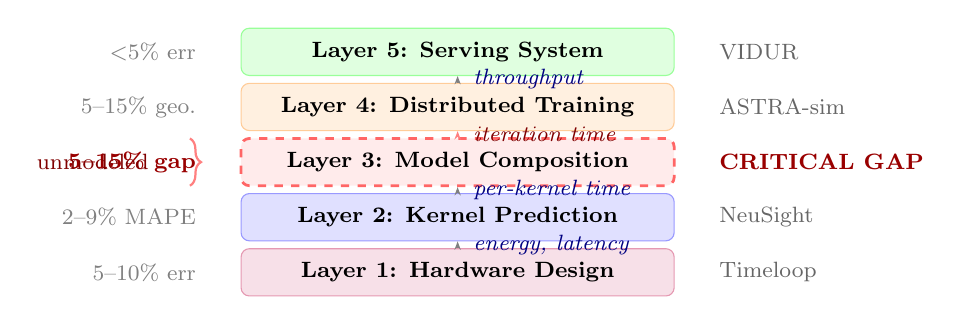
\begin{tikzpicture}[layer/.style={draw=black!60, rounded corners=3pt, minimum width=5.5cm, minimum height=0.6cm, align=center, font=\footnotesize\bfseries}, tool/.style={font=\footnotesize, text=black!60}, arr/.style={-{Stealth[length=3pt]}, thick, black!50}, data/.style={font=\footnotesize\itshape, text=blue!50!black}]
\node[layer, fill=purple!12, draw=purple!40] (hw) at (0,0) {Layer 1: Hardware Design}; \node[tool, anchor=west] at (3.2,0) {Timeloop}; \node[layer, fill=blue!12, draw=blue!40] (kernel) at (0,0.7) {Layer 2: Kernel Prediction}; \node[tool, anchor=west] at (3.2,0.7) {NeuSight}; \node[layer, fill=red!8, draw=red!60, dashed, line width=1pt] (comp) at (0,1.4) {Layer 3: Model Composition}; \node[font=\footnotesize\bfseries, text=red!60!black, anchor=west] at (3.2,1.4) {CRITICAL GAP}; \node[layer, fill=orange!12, draw=orange!40] (dist) at (0,2.1) {Layer 4: Distributed Training}; \node[tool, anchor=west] at (3.2,2.1) {ASTRA-sim}; \node[layer, fill=green!12, draw=green!40] (serve) at (0,2.8) {Layer 5: Serving System}; \node[tool, anchor=west] at (3.2,2.8) {VIDUR};
\draw[arr] (hw) -- node[data, right, xshift=2pt] {energy, latency} (kernel); \draw[arr] (kernel) -- node[data, right, xshift=2pt] {per-kernel time} (comp); \draw[arr, draw=red!50, dashed] (comp) -- node[data, right, xshift=2pt, text=red!50!black] {iteration time} (dist); \draw[arr] (dist) -- node[data, right, xshift=2pt] {throughput} (serve);
\node[font=\footnotesize, text=black!50, anchor=east] at (-3.2,0) {5--10\% err}; \node[font=\footnotesize, text=black!50, anchor=east] at (-3.2,0.7) {2--9\% MAPE}; \node[font=\footnotesize, text=red!60!black, anchor=east] at (-3.2,1.4) {\textbf{5--15\% gap}}; \node[font=\footnotesize, text=black!50, anchor=east] at (-3.2,2.1) {5--15\% geo.}; \node[font=\footnotesize, text=black!50, anchor=east] at (-3.2,2.8) {$<$5\% err}; \draw[decorate, decoration={brace, amplitude=4pt, mirror}, thick, red!50] (-3.4,1.1) -- (-3.4,1.7); \node[font=\footnotesize, text=red!50!black, anchor=east] at (-3.8,1.4) {unmodeled};
\end{tikzpicture}}\caption{Unified five-layer pipeline. Layer~3 (dashed) is the critical unmodeled gap.}\label{fig:pipeline-architecture}\end{figure}
\section{Open Challenges and Future Directions}\label{sec:challenges}
\textbf{(1)~Composition gap:} Kernel errors of 2--3\% yield 5--12\% model-level error (Figure~\ref{fig:error-composition}) with no validated pipeline. \textbf{(2)~Frontier workloads:} MoE, diffusion~\cite{dynamicreasoning2026}, and dynamic inference lack validated tools; scaling laws~\cite{kaplan2020scaling,hoffmann2022chinchilla,scalinglawguide2025,scalinglaws2024} predict loss but not latency (Figure~\ref{fig:workload-coverage}).
\begin{figure}[t]
\centering\resizebox{\columnwidth}{!}{%
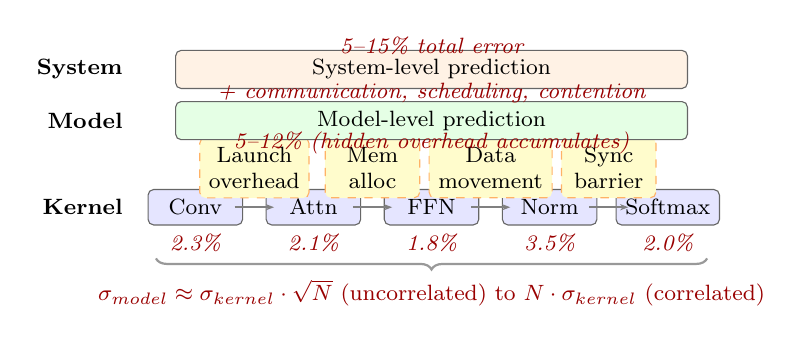
\begin{tikzpicture}[box/.style={draw=black!60, rounded corners=2pt, minimum width=1.2cm, minimum height=0.45cm, align=center, font=\footnotesize}, err/.style={font=\footnotesize\itshape, text=red!60!black}, arr/.style={-{Stealth[length=3pt]}, thick, black!50}, brace/.style={decorate, decoration={brace, amplitude=4pt, mirror}, thick, black!40}]
\node[box, fill=blue!10] (k1) at (0,0) {Conv}; \node[box, fill=blue!10] (k2) at (1.5,0) {Attn}; \node[box, fill=blue!10] (k3) at (3,0) {FFN}; \node[box, fill=blue!10] (k4) at (4.5,0) {Norm}; \node[box, fill=blue!10] (k5) at (6,0) {Softmax}; \node[err] at (0,-0.45) {2.3\%}; \node[err] at (1.5,-0.45) {2.1\%}; \node[err] at (3,-0.45) {1.8\%}; \node[err] at (4.5,-0.45) {3.5\%}; \node[err] at (6,-0.45) {2.0\%}; \node[font=\footnotesize\bfseries, anchor=east] at (-0.8,0) {Kernel}; \draw[arr] (0.5,0) -- (1,0); \draw[arr] (2,0) -- (2.5,0); \draw[arr] (3.5,0) -- (4,0); \draw[arr] (5,0) -- (5.5,0);
\node[box, fill=yellow!20, dashed, draw=orange!60] (h1) at (0.75,0.5) {Launch\\overhead}; \node[box, fill=yellow!20, dashed, draw=orange!60] (h2) at (2.25,0.5) {Mem\\alloc}; \node[box, fill=yellow!20, dashed, draw=orange!60] (h3) at (3.75,0.5) {Data\\movement}; \node[box, fill=yellow!20, dashed, draw=orange!60] (h4) at (5.25,0.5) {Sync\\barrier};
\node[box, fill=green!10, minimum width=6.5cm] (model) at (3,1.1) {Model-level prediction}; \node[err] at (3,0.82) {5--12\% (hidden overhead accumulates)}; \node[font=\footnotesize\bfseries, anchor=east] at (-0.8,1.1) {Model}; \node[box, fill=orange!10, minimum width=6.5cm] (system) at (3,1.75) {System-level prediction}; \node[err] at (3,1.45) {+ communication, scheduling, contention}; \node[font=\footnotesize\bfseries, anchor=east] at (-0.8,1.75) {System}; \node[err] at (3,2.05) {5--15\% total error};
\draw[brace] (-0.5,-0.65) -- (6.5,-0.65) node[midway, below=4pt, font=\footnotesize, text=red!60!black] {$\sigma_{\text{model}} \approx \sigma_{\text{kernel}} \cdot \sqrt{N}$ (uncorrelated) to $N \cdot \sigma_{\text{kernel}}$ (correlated)};
\end{tikzpicture}}\caption{Error composition: kernel predictions (2--3\%) accumulate to 5--15\% at system level.}\label{fig:error-composition}\end{figure}
\begin{figure}[t]
\centering\resizebox{\columnwidth}{!}{%
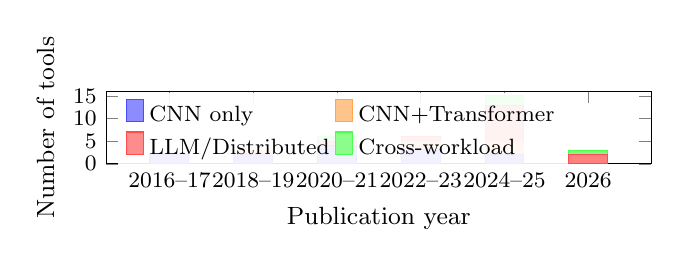
\begin{tikzpicture}
\begin{axis}[ybar stacked, bar width=14pt, xlabel={Publication year}, ylabel={Number of tools}, ymin=0, ymax=16, xtick={2016,2018,2020,2022,2024,2026}, xticklabels={2016--17,2018--19,2020--21,2022--23,2024--25,2026}, xticklabel style={font=\footnotesize}, yticklabel style={font=\footnotesize}, xlabel style={font=\small}, ylabel style={font=\small}, legend style={at={(0.02,0.98)}, anchor=north west, font=\footnotesize, draw=none, fill=white, fill opacity=0.9, text opacity=1, legend columns=2}, legend cell align={left}, height=2.5cm, width=8.5cm, enlarge x limits={abs=0.8cm}]
\addplot[fill=blue!50, draw=blue!70] coordinates {(2016,2) (2018,2) (2020,4) (2022,3) (2024,2) (2026,0)}; \addplot[fill=orange!50, draw=orange!70] coordinates {(2016,0) (2018,1) (2020,0) (2022,2) (2024,3) (2026,0)}; \addplot[fill=red!50, draw=red!70] coordinates {(2016,0) (2018,0) (2020,1) (2022,1) (2024,8) (2026,2)}; \addplot[fill=green!50, draw=green!70] coordinates {(2016,0) (2018,0) (2020,1) (2022,0) (2024,2) (2026,1)};
\legend{CNN only, CNN+Transformer, LLM/Distributed, Cross-workload}
\end{axis}\end{tikzpicture}}\caption{Workload coverage by publication period. MoE and diffusion models remain uncharacterized.}\label{fig:workload-coverage}\end{figure}
\textbf{(3)~Hardware transfer:} Cross-family transfer (GPU$\rightarrow$TPU$\rightarrow$PIM~\cite{upimulator2024,attacc2024,neupims2024,paise2025}) and congestion modeling~\cite{astrasim2023,triosim2025} remain unsolved. \textbf{(4)~Standardized evaluation:} No MLPerf~\cite{mlperf_training2020,mlperf_inference2020,mlperfpower2025} equivalent exists for simulators; portable formats~\cite{chakra2023} and continuous validation are needed; concurrent surveys~\cite{svedassurvey2025} similarly identify this gap. \textbf{(5)~Reproducibility:} nn-Meter failed from dependency rot; containerization and CI testing are needed. \textbf{(6)~Software stack evolution:} Rapidly evolving optimizations such as FlashAttention~\cite{flashattention2022} invalidate performance models trained on prior kernel implementations.
\section{Conclusion}\label{sec:conclusion}
We survey 25 ML performance tools and evaluate ten against a 36-scenario benchmark, finding self-reported accuracy unreliable (NeuSight: 2.3\% claimed vs.\ 5.87--27.10\%; nn-Meter: no output). The 5--15\% composition gap dominates total error; closing it requires validated composition models and community CI.
\bibliographystyle{ACM-Reference-Format}
\bibliography{references}
\end{document}
